\documentclass[11pt,class=report,crop=false]{standalone}
\usepackage[screen]{../python}

\begin{document}


%====================================================================
\chapitre{Graphes et combinatoire de Ramsey}
%====================================================================

\objectifs{Tu vas voir qu'un problème tout simple, qui concerne les relations entre seulement six personnes, va demander énormément de calculs pour être résolu.}

\begin{center}
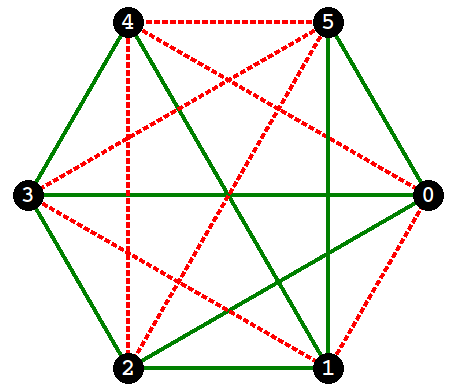
\includegraphics[scale=\myscale,scale=0.4]{ecran-ramsey-1d}
\end{center} 

\index{graphe}


\insertvideo{CsCSRszXYxI}{Graphe et combinatoire de Ramsey}


%%%%%%%%%%%%%%%%%%%%%%%%%%%%%%%%%%%%%%%%%%%%%%%%%%%%%%%%%%%%%%%%
%%%%%%%%%%%%%%%%%%%%%%%%%%%%%%%%%%%%%%%%%%%%%%%%%%%%%%%%%%%%%%%%

\begin{cours}[Le problème de Ramsey]

\objectifs{Proposition. Dans un groupe de $6$ personnes, il y a toujours $3$ amis (les trois se connaissent deux à deux) ou $3$ étrangers (les trois sont tous des inconnus les uns pour les autres).}

Le but de cette fiche est de faire démontrer à l'ordinateur cet énoncé. Pour cela nous allons modéliser le problème par des graphes, puis nous allons vérifier l'énoncé pour chacun des $32\,768$ graphes possibles.

\bigskip 

On considère $n$ personnes. Pour deux personnes parmi elles, soit elles se connaissent (elles sont amies), soit elles ne se connaissent pas (elles sont étrangères l'une à l'autre). Nous schématisons cela par un graphe :
\begin{itemize}
  \item une personne est représentée par un sommet (numéroté de $0$ à $n-1$) ;
  \item si deux personnes sont amies, on relie les sommets correspondants par une arête verte ;
  \item sinon (elles sont étrangères), on relie les sommets correspondants par une arête pointillée rouge. 
\end{itemize}

Le graphe ci-dessous signifie que $0$ est ami avec $2$ ; $1$ est ami avec $3$. Les autres paires ne se connaissent pas.
\myfigure{0.8}{
  \tikzinput{fig-ramsey-0a}
}

Un graphe vérifie le problème de Ramsey, s'il y a parmi ses sommets, ou bien $3$ amis, ou bien s'il y a $3$ étrangers.
\myfigure{0.4}{
  \tikzinput{fig-ramsey-0b}
}

Voici un exemple de graphe à $5$ sommets qui vérifie l'énoncé : il possède bien $3$ sommets étrangers (les sommets $0$, $2$ et $4$), même s'il ne possède pas trois amis.

\myfigure{0.5}{
  \tikzinput{fig-ramsey-0c}
}
\end{cours}


\begin{cours}[Modélisation]


\objectifs{Nous modélisons un graphe par un tableau à double entrée, contenant des $0$ et des $1$.}

Soit un graphe ayant $n$ sommets, numérotés de $0$ à $n-1$.
Le \defi{tableau du graphe} est un tableau de taille $n \times n$ dans lequel on place un $1$ en position $(i,j)$ si les sommets $i$ et $j$ sont reliés par une arête, sinon on place un $0$.

\bigskip
Premier exemple ci-dessous : les sommets $0$ et $2$ sont amis (car reliés par un arête verte) donc le tableau contient un $1$ en position $(0,2)$ et aussi en $(2,0)$. De même $1$ et $3$ sont amis, donc le tableau contient un $1$ en position $(1,3)$ et $(3,1)$. Le reste du tableau contient des $0$.

\myfigure{0.7}{
  \tikzinput{fig-ramsey-1a}
}

Voici un graphe plus compliqué et son tableau :
\myfigure{0.7}{
  \tikzinput{fig-ramsey-1c}
}

\end{cours}



%%%%%%%%%%%%%%%%%%%%%%%%%%%%%%%%%%%%%%%%%%%%%%%%%%%%%%%%%%%%%%%%
% Activité 1
%%%%%%%%%%%%%%%%%%%%%%%%%%%%%%%%%%%%%%%%%%%%%%%%%%%%%%%%%%%%%%%%

\begin{activite}[Construire des graphes]

\objectifs{Objectifs : définir des graphes et tester si trois sommets donnés sont amis.}


\begin{center}
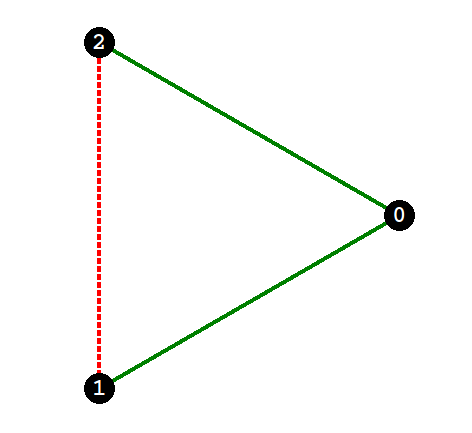
\includegraphics[scale=\myscale,height=5cm]{ecran-ramsey-1a}\quad
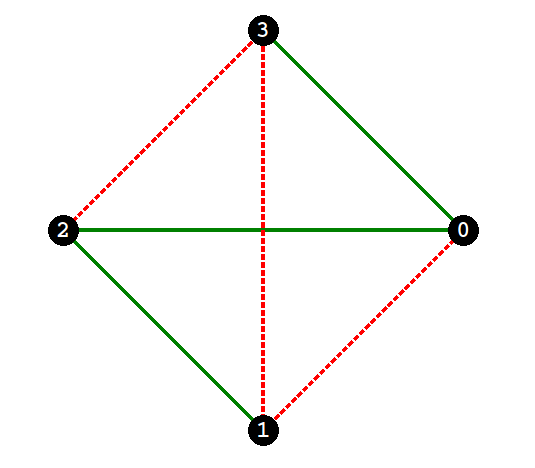
\includegraphics[scale=\myscale,height=5cm]{ecran-ramsey-1b}
\end{center} 
\begin{center}
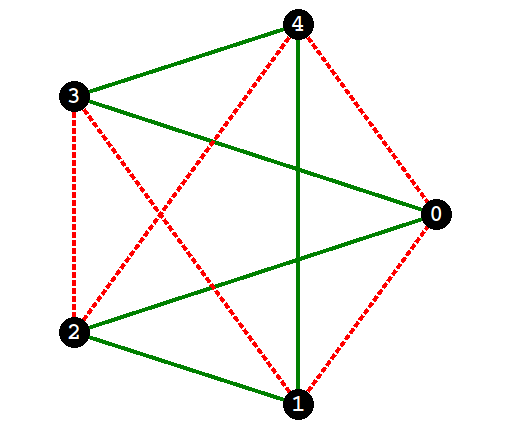
\includegraphics[scale=\myscale,height=5cm]{ecran-ramsey-1c}\quad
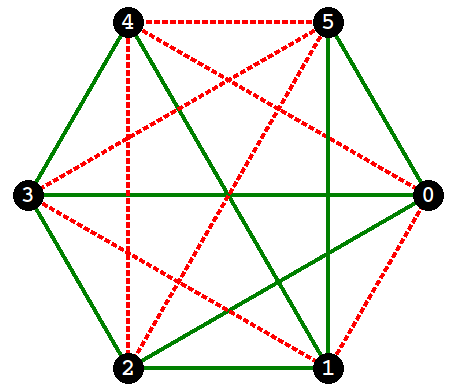
\includegraphics[scale=\myscale,height=5cm]{ecran-ramsey-1d}
\end{center} 


\begin{enumerate}
  \item Définis le tableau des graphes des quatre exemples ci-dessus.
  Tu peux commencer par initialiser le tableau par \\
  \centerline{\ci{graphe = [[0 for j in range(n)] for i in range(n)]}}
  Puis ajoute des commandes :\\
  \centerline{\ci{graphe[i][j] = 1} \quad et \quad \ci{graphe[j][i] = 1}}
  
  N'oublie pas que si le sommet $i$ est relié au sommet $j$ par une arête, alors il faut mettre un $1$ en position $(i,j)$ mais aussi en position $(j,i)$. 
  
  \item Définis une fonction \ci{voir_graphe(graphe)} qui permet d'afficher à l'écran le tableau d'un graphe.
  Ainsi le troisième exemple ci-dessus (avec $n=5$) doit s'afficher ainsi :
\begin{center}
\ci{00110}\\
\ci{00101}\\
\ci{11000}\\
\ci{10001}\\
\ci{01010}\\
\end{center}

  \item On fixe trois sommets $i$, $j$, $k$ d'un graphe. Écris une fonction \ci{contient_3_amis_fixes(graphe,i,j,k)} qui teste si les sommets $i$, $j$, $k$ sont trois amis (la fonction renvoie \og{}vrai\fg{} ou \og{}faux\fg{}). Fais le même travail avec une fonction \ci{contient_3_etrangers_fixes(graphe,i,j,k)} pour savoir si ces sommets sont étrangers.
  
Trouve à la main sur le quatrième exemple, trois sommets amis ou étrangers et vérifie ta réponse à l'aide des fonctions que tu viens de définir.

\end{enumerate}   
     
\end{activite}


%%%%%%%%%%%%%%%%%%%%%%%%%%%%%%%%%%%%%%%%%%%%%%%%%%%%%%%%%%%%%%%%
% Activité 2
%%%%%%%%%%%%%%%%%%%%%%%%%%%%%%%%%%%%%%%%%%%%%%%%%%%%%%%%%%%%%%%%

\begin{activite}[Afficher des jolis graphes]

\objectifs{Objectifs : dessiner un graphe ! Activité facultative.}

\begin{center}
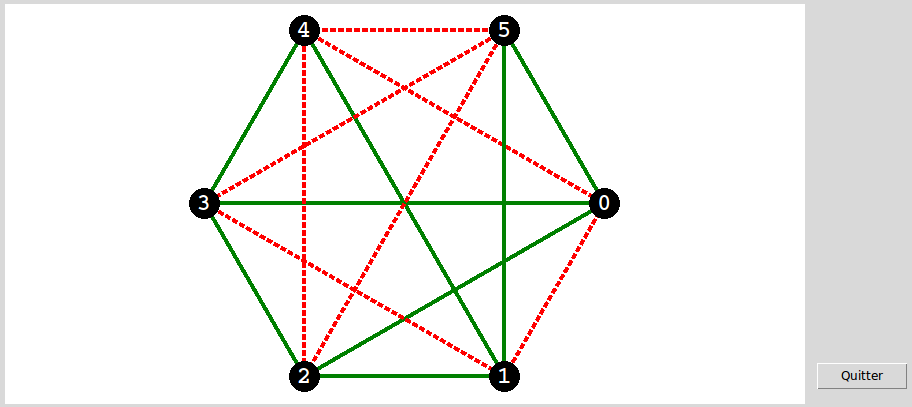
\includegraphics[scale=\myscale,scale=0.4]{ecran-ramsey-2}
\end{center}

Programme l'affichage graphique d'un graphe par une fonction \ci{afficher_graphe(graphe)}.
     
\bigskip
     
\emph{Indications.} Cette activité n'est pas nécessaire pour la suite, elle aide juste à visualiser les graphes. Il faut utiliser le module \ci{tkinter} et les fonctions \ci{create_line()}, \ci{create_oval()} et éventuellement \ci{create_text()}. 
% Voir les fiches précédentes.

Le point le plus délicat est d'obtenir les coordonnées des sommets. Tu auras besoin des fonctions sinus et cosinus (disponibles dans le module \ci{math}).
Les coordonnées $(x_i,y_i)$ du sommet numéro $i$ d'un graphe à $n$ éléments peuvent être calculées par les formules :
$$x_i = r \cos\left(\frac{2 i \pi}{n}\right) \qquad \text{ et } \qquad y_i = r\sin\left(\frac{2 i \pi}{n}\right).$$

Ces sommets sont situés sur le cercle de rayon $r$, centré en $(0,0)$. 
Tu devras choisir $r$ assez grand (par exemple $r=200$) et décaler le cercle pour bien l'afficher à l'écran.


\myfigure{0.7}{
  \tikzinput{fig-ramsey-2}
}
\end{activite}

%%%%%%%%%%%%%%%%%%%%%%%%%%%%%%%%%%%%%%%%%%%%%%%%%%%%%%%%%%%%%%%%
% Activité 3
%%%%%%%%%%%%%%%%%%%%%%%%%%%%%%%%%%%%%%%%%%%%%%%%%%%%%%%%%%%%%%%%

\begin{activite}[Écriture binaire avec des $0$ non significatifs]

\objectifs{Objectifs : convertir un entier en écriture binaire avec éventuellement des zéros non significatifs.}

\index{binaire}
\index{ecriture@écriture!binaire}

Programme une fonction \ci{decimal_vers_binaire(p,n)} qui affiche l'écriture binaire d'un entier $p$ sur $n$ \emph{bits}. Le résultat est une liste de $0$ et de $1$.

\bigskip

Exemple.
\begin{itemize}
  \item L'écriture binaire de $p=37$ est $1.0.0.1.0.1$. Si on veut 
son écriture binaire sur $n=8$ \emph{bits} alors il faut rajouter deux $0$ non significatifs devant : $0.0.1.0.0.1.0.1$. 
  \item Ainsi le résultat de la commande \ci{decimal_vers_binaire(37,8)} doit être \ci{[0, 0, 1, 0, 0, 1, 0, 1]}.
  \item 
La commande \ci{decimal_vers_binaire(37,10)} renvoie l'écriture de $37$ en binaire sur $10$ \emph{bits} : \ci{[0, 0, 0, 0, 1, 0, 0, 1, 0, 1]}.
\end{itemize}

\bigskip

\emph{Indications.}
\begin{itemize}
  \item Tu peux utiliser la commande \ci{bin(p)} !
  \item La commande \ci{list(ma_chaine)}\index{list@\ci{list}}\index{chaine@chaîne!caracteres@caractères} renvoie la liste des caractères composant \ci{ma_chaine}.
  \item Attention ! On veut une liste d'entiers \ci{0} ou \ci{1}, pas des caractères \ci{'0'} ou \ci{'1'}. La commande \ci{int('0')} renvoie \ci{0} et \ci{int('1')} renvoie \ci{1}.
  
  \item \ci{ma_liste = ma_liste + [element]} ajoute un élément en fin de liste, alors que \ci{ma_liste = [element] + ma_liste} ajoute l'élément en début de liste.
\end{itemize} 
  
\end{activite}


%%%%%%%%%%%%%%%%%%%%%%%%%%%%%%%%%%%%%%%%%%%%%%%%%%%%%%%%%%%%%%%%
% Activité 4
%%%%%%%%%%%%%%%%%%%%%%%%%%%%%%%%%%%%%%%%%%%%%%%%%%%%%%%%%%%%%%%%

\begin{cours}[Sous-ensembles]

Soit $E_n = \{0,1,2,\ldots,n-1\}$ l'ensemble des entiers de $0$ à $n-1$. L'ensemble $E_n$ contient donc $n$ éléments.

Par exemple $E_3 = \{ 0,1,2 \}$, $E_4 = \{ 0,1,2,3 \}$\ldots

\bigskip

\textbf{Sous-ensembles.}

Quels sont les sous-ensembles de $E_n$ ? Par exemple il y a $8$ sous-ensembles de $E_3$, ce sont :
    \begin{itemize}
      \item le sous-ensemble $\{0\}$ composé du seul élément $0$ ;
      \item le sous-ensemble $\{1\}$ composé du seul élément $1$ ;      
      \item le sous-ensemble $\{2\}$ composé du seul élément $2$ ; 
      \item le sous-ensemble $\{0,1\}$ composé de l'élément $0$ et de l'élément $1$ ;           
      \item le sous-ensemble $\{0,2\}$ ;
      \item le sous-ensemble $\{1,2\}$ ; 
      \item le sous-ensemble $\{0, 1,2\}$ composé de tous les éléments ;
      \item l'ensemble vide $\varnothing$ qui ne contient aucun élément !    
    \end{itemize} 

\medskip

\textbf{Proposition.} L'ensemble $E_n$ contient $2^n$ sous-ensembles.

\medskip

Par exemple $E_4 = \{ 0,1,2,3 \}$ possède $2^4 = 16$ sous-ensembles possibles. Amuse-toi à les trouver tous ! Pour $E_6$ il y a $2^6 = 64$  sous-ensembles possibles.

\bigskip

\textbf{Sous-ensembles de cardinal fixé.}

On cherche seulement les sous-ensembles ayant un nombre $k$ fixé d'éléments.

Exemples :
\begin{itemize}
  \item Pour $n = 3$ et $k = 2$, les sous-ensembles à deux éléments contenus dans $E_3 = \{ 0,1,2 \}$ sont les trois paires : $\{0,1\}$, $\{0,2\}$, $\{1,2\}$.

  \item Pour $n = 5$ et $k = 3$, les sous-ensembles à trois éléments contenus dans $E_5 = \{ 0,1,2,3,4 \}$ sont les $10$ triplets :
  $\{0, 1, 2\}$, $\{0, 1, 3\}$, $\{0, 2, 3\}$, $\{1, 2, 3\}$, $\{0, 1, 4\}$, $\{0, 2, 4\}$, $\{1, 2, 4\}$, $\{0, 3, 4\}$, $\{1, 3, 4\}$, $\{2, 3, 4\}$.
  
\end{itemize}

\end{cours}


\begin{activite}[Sous-ensembles]

\objectifs{Objectifs : générer tous les sous-ensembles afin de tester tous les triplets de sommets. Pour cela nous utiliserons l'écriture binaire.}

Voici comment nous associons à chaque entier $p$ vérifiant $0 \le p < 2^n$ un sous-ensemble de $E_n = \{0,1,\ldots, n-1\}$.

Commençons par un exemple, avec $n = 6$ et $p=26$ :
\begin{itemize}
  \item l'écriture binaire de $p=26$ sur $n=6$ \emph{bits} est 
  \ci[0,1,1,0,1,0] ;
  \item il y a des $1$ au rang $1$, $2$ et $4$ (en commençant au rang $0$ à gauche) ;
  \item le sous-ensemble associé est alors $\{1,2,4\}$.
\end{itemize}


\myfigure{0.7}{
  \tikzinput{fig-ramsey-4a}
}


\bigskip

Autres exemples.
\begin{itemize}
  \item Avec $n = 8$ et $p = 57$ dont l'écriture binaire sur $8$ \emph{bits} est \ci{[0,0,1,1,1,0,0,1]}, le sous-ensemble associé correspond aux rangs $2,3,4,7$, c'est donc $\{2,3,4,7\}$.
  
  \smallskip
  
\myfigure{0.6}{
  \tikzinput{fig-ramsey-4b}
}  

  
  \item Avec $p=0$, l'écriture binaire est formée uniquement de $0$, le sous-ensemble associé est l'ensemble vide.
  \item Avec $p = 2^n - 1$, l'écriture binaire est formée uniquement de $1$, le sous-ensemble associé est $E_n = \{0,1,\ldots, n-1\}$ tout entier.
\end{itemize}

\bigskip

Nous modélisons un ensemble comme une liste d'éléments.
Par exemple :
\begin{itemize}
  \item L'ensemble $E_4$ est pour nous la liste \ci{[0,1,2,3]}.
  \item Un sous-ensemble de $E_4$ est par exemple la paire \ci{[1,3]}.
  \item L'ensemble vide est représenté par la liste vide \ci{[]}.
\end{itemize}



\begin{enumerate}
  \item Programme la fonction \ci{sous_ensembles(n)} qui renvoie la liste de tous les sous-ensembles possibles de $E_n =  \{0,1,2,\ldots,n-1\}$.
  
  Par exemple, pour $n=3$, \ci{sous_ensembles(n)} renvoie la liste (qui contient elle-même des listes) :\\
\centerline{\ci{[ [], [2], [1], [1, 2], [0], [0, 2], [0, 1], [0, 1, 2]  ]}}
C'est-à-dire les $8$ sous-ensembles (en commençant par l'ensemble vide) :
$$\varnothing \quad \{2\}\quad \{1\}\quad \{1,2\}\quad \{0\}\quad \{0,2\}\quad \{0,1\}\quad \{0,1,2\}.$$

\emph{Indication.} Pour tester ton programme, vérifie que la liste renvoyée contient bien $2^n$ sous-ensembles.

  \item Déduis-en une fonction \ci{sous_ensembles_fixe(n,k)} qui renvoie seulement les sous-ensembles de $E_n$ ayant $k$ éléments.
  
 Par exemple, pour $n=3$ et $k=2$, \ci{sous_ensembles_fixe(n,k)} renvoie la liste des paires :\\
\centerline{\ci{[ [0, 1], [0, 2], [1, 2] ]}}
 
Teste ton programme :
\begin{itemize}
  \item Pour $n=4$ et $k=3$, la liste renvoyée par \ci{sous_ensembles_fixe(n,k)} contient $4$ triplets.
  \item Pour $n=5$ et $k=3$, il y a $10$ triplets possibles.
  \item Pour $n=10$ et $k=4$, il y a $210$ sous-ensembles possibles !
\end{itemize}

\end{enumerate}  


Dans la suite nous utiliserons surtout les sous-ensembles à $3$ éléments.
En particulier, pour $n=6$, les triplets inclus dans $\{0,1,2,3,4,5\}$ sont au nombre de $20$ :
\begin{center}
\ci{[[3, 4, 5], [2, 4, 5], [2, 3, 5], [2, 3, 4], [1, 4, 5], }
\ci{ [1, 3, 5], [1, 3, 4], [1, 2, 5], [1, 2, 4], [1, 2, 3],}
\ci{ [0, 4, 5], [0, 3, 5], [0, 3, 4], [0, 2, 5], [0, 2, 4], }
\ci{ [0, 2, 3], [0, 1, 5], [0, 1, 4], [0, 1, 3], [0, 1, 2]]}
\end{center}
   
\end{activite}

%%%%%%%%%%%%%%%%%%%%%%%%%%%%%%%%%%%%%%%%%%%%%%%%%%%%%%%%%%%%%%%%
% Activité 5
%%%%%%%%%%%%%%%%%%%%%%%%%%%%%%%%%%%%%%%%%%%%%%%%%%%%%%%%%%%%%%%%

\begin{activite}[Théorème de Ramsey pour $n=6$]

\objectifs{Objectifs : vérifier que tous les graphes ayant $6$ sommets contiennent trois amis ou bien trois étrangers.}

\begin{enumerate}
  \item Programme une fonction \ci{graphe_contient_3(graphe)} qui teste si un graphe contient $3$ amis ou bien $3$ étrangers. Il faut donc appeler les fonctions \ci{contient_3_amis_fixes(graphe,i,j,k)} et \ci{contient_3_etrangers_fixes(graphe,i,j,k)} de la première activité pour tous les triplets possibles de sommets $(i,j,k)$.
 
 Pour les quatre exemples de la première activité, seul le quatrième (avec $6$ sommets) vérifie le test.
  
  \item Programme une fonction \ci{voir_tous_graphes(n)} qui affiche tous les tableaux possibles de graphes à $n$ sommets.
  Il y a $N = \frac{(n-1)n}{2}$ tableaux possibles. Tu peux les générer par une méthode similaire à celle pour les sous-ensembles :
  \begin{itemize}
    \item pour chaque entier $p$ qui vérifie $0 \le p < 2^N$,
    \item calcule l'écriture binaire de $p$ sur $N$ \emph{bits},
    \item remplis le tableau élément par élément, avec les $0$ et les $1$ de l'écriture binaire.
  \end{itemize}


\emph{Indications.}
Pour remplir un tableau à partir d'une écriture binaire \ci{b} donnée, tu peux utiliser une double boucle du type :

\begin{lstlisting}
for j in range(0,n):
    for i in range(j+1,n):
        b = liste_binaire.pop()
        graphe[i][j] = b
        graphe[j][i] = b
\end{lstlisting}
  
Voici le principe de cette boucle qui remplit la partie au-dessus de la diagonale (et aussi la partie en-dessous par symétrie).
Cette boucle prend le dernier \emph{bit} de la liste et le place sur la première case libre au-dessus de la diagonale ; puis l'avant-dernier \emph{bit} est placé sur la seconde case libre\ldots ; le premier \emph{bit} de la liste remplit la dernière case libre.


 \myfigure{0.8}{
  \tikzinput{fig-ramsey-5}
} 
  
  \item Transforme la fonction précédente en une fonction \ci{test_tous_graphes(n)}
qui teste la conjecture \og{}il y a trois amis ou trois étrangers\fg{} pour tous les graphes à $n$ sommets.
Tu dois trouver que :
\begin{itemize}
\item pour $n=4$ et $n=5$ la conjecture est fausse. Donne un graphe à $4$ sommets (puis à $5$ sommets) qui n'a ni $3$ amis, ni $3$ étrangers ;
\item pour $n=6$ laisse l'ordinateur vérifier que, pour chacun des $N = 2^{\frac{5 \times 6}{2}} = 32\,768$ graphes ayant $6$ sommets, soit il possède $3$ amis, soit il possède $3$ étrangers.
\end{itemize}
\end{enumerate}   
     
\end{activite}


\begin{activite}[Pour aller plus loin]

\objectifs{Objectifs : améliorer ton programme et prouver d'autres conjectures. Activité facultative.}

\begin{enumerate}
  \item Améliore ton programme afin qu'il vérifie la conjecture pour $n=6$ en moins d'une seconde.
  
  
\emph{Idées.}
  \begin{itemize}
    \item Il faut générer la liste des triplets une fois pour toute au début du programme (et non à chaque nouveau graphe).
    \item Il ne faut pas générer une liste de tous les graphes possibles, puis les tester dans un second temps. Il faut en générer un puis le tester avant de passer au suivant.
    \item Dès que tu as trouvé $3$ amis (ou $3$ étrangers) c'est gagné ! Stoppe immédiatement la boucle quitte à utiliser l'instruction \ci{break} et passe au graphe suivant.
    \item Tu peux seulement tester les graphes qui correspondent à $p$ entre $0$ et $2^{N}/2$ (car pour les $p$ suivants cela revient à échanger les segments verts en rouges et inversement).
  \end{itemize}
  
\medskip
  
  Avec ces conseils voici les temps de calcul auxquels tu peux t'attendre :
  \begin{center}
  \begin{tabular}{|c|c|c|}
  \hline
  Nombre de sommets & Nombre de graphes & Temps de calcul approximatif \\
  \hline\hline
  $n=6$ & 32\,768 & $< 1$ seconde \\
  $n=7$ & 2\,097\,152 & $< 1$ minute \\  
  $n=8$ & 268\,435\,456 & $< 1$ heure \\
  $n=9$ & 68\,719\,476\,736 & $< 10$ jours \\ 
  \hline
  \end{tabular} 
  \end{center}




 
  \item Il existe un énoncé plus difficile. Il s'agit de trouver à partir de quelle taille $n$ un graphe contient toujours ou bien $4$ amis ou bien $3$ étrangers. 
  \^Etre $4$ amis signifie que deux à deux ils sont reliés par un segment vert, comme ci-dessous :
  \myfigure{1}{
  \tikzinput{fig-ramsey-6}
}  

  \begin{enumerate}
    \item Trouve des graphes à $n=6$ (puis $n=7$) sommets qui ne vérifient pas cet énoncé.
    \item En cherchant un peu avec la machine trouve des graphes à $8$ sommets qui ne vérifient pas cet énoncé.
    \item Prouve que n'importe quel graphe ayant $9$ sommets contient $4$ amis ou bien $3$ étrangers ! 
     
  \emph{Indications.} Il faut tester tous les graphes correspondants aux entiers $p$ compris entre $0$ et $2^N = 2^{\frac{8 \times 9}{2}} = 68\,719\,476\,736$. Le temps total de calcul est d'environ 20 jours ! Tu peux partager les calculs entre plusieurs ordinateurs : un ordinateur fait les calculs pour $0 \le p \le 1\,000\,000$, un deuxième ordinateur pour $1\,000\,001 \le p \le 2\,000\,000$,\ldots
    
  \end{enumerate}
  
  \item 
  \begin{itemize}
    \item   Il existe des raisonnements pour pouvoir démontrer à la main que pour $n=6$ il y a toujours $3$ amis ou $3$ étrangers. Cherche un tel raisonnement ! Avec un peu plus d'efforts, on prouve aussi que c'est $n=9$ qui répond au problème des $4$ amis/$3$ étrangers.
    
    \item On sait prouver qu'il faut $n=18$ sommets pour avoir toujours $4$ amis ou $4$ étrangers.
    
    \item Par contre personne dans le monde ne sait quelle est la valeur du plus petit $n$ pour le problème des $5$ amis/$5$ étrangers !
  \end{itemize}

\end{enumerate}

\end{activite}

%%%%%%%%%%%%%%%%%%%%%%%%%%%%%%%%%%%%%%%%%%%%%%%%%%%%%%%%%%%%%%%%
% Corrections
%%%%%%%%%%%%%%%%%%%%%%%%%%%%%%%%%%%%%%%%%%%%%%%%%%%%%%%%%%%%%%%%
%
%
%\footnotesize
%
%\begin{multicols}{2}[\section*{Corrections}]
%
%\begin{code}[Activité 1]
%\soustitre{Question 1}
%\begin{lstlisting}
%pass
%\end{lstlisting}
%\end{code}
%
%\end{multicols}

\end{document}
